\documentclass[revision-guide.tex]{subfiles}
%% Current Author: CJRU
\setcounter{chapter}{14}
\begin{document}
\chapter{Special Relativity}

This chapter contains revision on the topics of:

\begin {itemize}
\item Einstein’s special principle of relativity
\item Time dilation
\item Length contraction

\end {itemize}

\textbf{Candidates should be able to:}
\spec{recall that Maxwell’s equations describe the electromagnetic field and predict the existence of electromagnetic waves that travel at the speed of light (Maxwell’s equations are not required)}

Maxwell related electricity and magnetism in a mathematically elegant way, and in doing so predicted that the speed of electromagnetic waves was:
\\
 
$c=\frac{1}{\sqrt{\epsilon_0\mu_0}}$ = 3 x 10$^8$ ms$^{-1}$



\spec{*recall that analogies with mechanical wave motion led most physicists to assume that electromagnetic
waves must be vibrations in an electromagnetic medium (the aether) filling absolute space}

Just what was it that was oscillating? Most physicists thought there must be a medium...

\spec{*recall that experiments to measure variations in the speed of light caused by the Earth’s motion
through the ether gave null results}

...However experiments such as the Michelson-Morley experiment\footnote{http://scienceworld.wolfram.com/physics/Michelson-MorleyExperiment.html} showed that there was no difference in the measurement of the speed of light over the course of a year - if the Earth was travelling through an aether you would expect the discrepancy to be measurable. But crucially no differences were found.


\spec{*understand that Einstein’s theory of special relativity dispensed with the aether and postulated that the
speed of light is a universal constant}

Einstein put forward the idea that there was no medium, and the speed of light was fixed.


\spec{*state the postulates of Einstein’s special principle of relativity}



His two postulates were 
\begin{itemize}
	\item The laws of physics are the same in all inertial rest frames
	\item The speed of light in free space is a fixed value
\end{itemize}

From these two postulates, it is possible to deduce the idea that time is not fixed for all observers, and that distances measured by two observers moving relative to each other may be different! A whole new avenue of physics was opened.

\spec{*explain how Einstein’s postulates lead to the idea of time dilation and length contraction that
undermines the idea of absolute time and space}

\subsection{Light clock}

Imagine a beam of light bouncing up and down between two mirrors, spaced a distance of 3 x 10$^8$ m apart

\begin{figure}[h]
	\begin{center}
		
		
		\begin{tikzpicture}
		\draw[very thick,black](-5.5,5) -- (-4.5,5);
		\draw[very thick, purple, -] (-5,0) -- node[left]{1 second between bounces}   (-5,5);
	 	\draw[very thick, purple, <->] (-5,1) --   (-5,4);
		\draw[very thick,black](-5.5,0) -- (-4.5,0);
	
		\end{tikzpicture}
		\end{center}
\end{figure}

Now imagine that you are moving right-to-left relative to the 'light clock' (or that the light clock is moving left-to-right relative to you - it doesn't matter...)


If the speed of light is constant for all observers, as Einstein's postulates require it will take longer between bounces, because it has to travel further due to the extra horizontal component:

 
\begin{figure}[h]
	\begin{center}	
		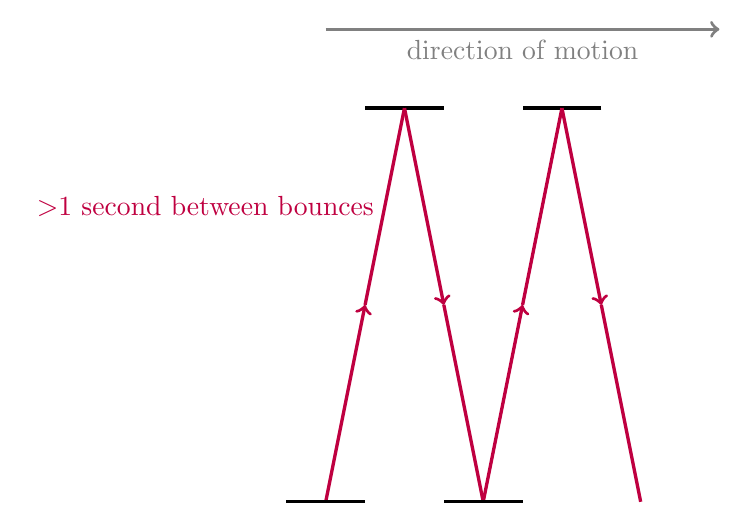
\begin{tikzpicture}
		\draw[very thick,black](-4.5,5) -- (-3.5,5);
		\draw[very thick, purple, ->] (-5,0) --   (-4.5,2.5);
		\draw[very thick, purple, -] (-4.5,2.5) -- node[left]{$>$1 second between bounces}   (-4,5);
		\draw[very thick,black](-5.5,0) -- (-4.5,0);
		\draw[very thick, purple, ->] (-4,5) --   (-3.5,2.5);
		\draw[very thick, purple, -] (-3.5,2.5) --   (-3,0);
		\draw[very thick,black](-1.5,5) -- (-2.5,5);
		\draw[very thick, purple, ->] (-3,0) --   (-2.5,2.5);
		\draw[very thick, purple, -] (-2.5,2.5) --   (-2,5);
		\draw[very thick,black](-2.5,0) -- (-3.5,0);
		\draw[very thick, purple, ->] (-2,5) --   (-1.5,2.5);
		\draw[very thick, purple, -] (-1.5,2.5) --   (-1,0);
		\draw[very thick, gray, ->] (-5,6) -- node[below]{direction of motion} (0,6);
		\end{tikzpicture}	
	\end{center}
\end{figure}



\spec{*recognise and use $t'=\frac{t}{\sqrt{1-\frac{v^2}{c^2}}}$ and $l'=l\sqrt{1-\frac{v^2}{c^2}}$}

\begin{example}

Cosmic radiation constantly bombards the Earth from outer space. The majority of these cosmic rays are protons which, when they hit the Earth’s upper atmosphere, create sub-atomic particles called pions, which then quickly decay into muons. Suppose a cosmic ray proton hits a molecule of nitrogen in the upper atmosphere at a distance of 50 km above the Earth’s surface. If the pion produced has a velocity of 0.9999c and has an average lifetime (in its own time) of t = $2.60 \times 10^{–8}\ $ s. How far would the pion travel before decaying taking into the effects of time dilation?

\answer 

First we must calculate the time it takes to decay according to a stationary observer. We do this by calculating the Lorentz factor $\gamma$ and multiplying this by the lifetime in its own frame of reference:

$\gamma = \frac{1}{\sqrt{1-\frac{v^2}{c^2}}} = 70.7$
\\
\\
so time taken to decay = 70.7 x 2.60 x 10$^{-8}$ = 1.83 x 10$^{-6}$ seconds
\\
Then distance travelled = speed x time = 550 m
\end{example}

\spec{*understand that two events which are simultaneous in one frame of reference may not be
simultaneous in another; explain this in terms of the fundamental postulates of relativity and distinguish
this from the phenomenon of time dilation}
\\

Imagine a situation in which a light is turned on in the middle of a train carriage, and light rays travel out in both forward and backwards directions. 
\\
\begin{figure}[h]
	\begin{center}
		
		
		\begin{tikzpicture}
		
		\draw (0,0) rectangle (10,5);
		\draw (2,0) circle (1);
		\draw (8,0) circle (1);
		\draw[very thick, purple, ->] (5.1,2.5) --   (8,2.5);
		\draw[very thick, purple, ->] (4.9,2.5) --   (2,2.5);
		
		
		\end{tikzpicture}
	\end{center}
\end{figure}
From the reference frame of a person riding along with the train, the light reaches each end of the carriage at the same time. Those events appear to be simultaneous.
\\
\begin{figure}[h]
	\begin{center}
		
		
		\begin{tikzpicture}
		
		\draw[very thick, gray, ->] (4,6) --   (6,6);
		\draw (2,0) rectangle (12,5);
		\draw (4,0) circle (1);
		\draw (10,0) circle (1);
		\draw[very thick, purple, ->] (5.1,2.5) --   (8,2.5);
		\draw[very thick, purple, ->] (4.9,2.5) --   (2,2.5);
		
		
		\end{tikzpicture}
	\end{center}
\end{figure}
In the reference frame of a stationary observer, the train is moving forward (to the right in this diagram), but the light rays travel at c, so the light ray travelling backwards will reach the rear end of the carriage first. 
\\

\begin{figure}[h]
	\begin{center}
		
		
		\begin{tikzpicture}
		
		\draw[very thick,gray, ->] (6,6) --   (4,6);
		\draw (-2,0) rectangle (8,5);
		\draw (0,0) circle (1);
		\draw (6,0) circle (1);
		\draw[very thick, purple, ->] (5.1,2.5) --   (8,2.5);
		\draw[very thick, purple, ->] (4.9,2.5) --   (2,2.5);
		
		
		\end{tikzpicture}
	\end{center}
\end{figure}
In the reference frame of somebody travelling faster than the train, the train appears to be going backwards, and the forward travelling light ray will reach the front end first. 
\\
The idea of two events being simultaneous is therefore impossible - it depends on your reference frame.
\\

This effect is  a completely different effect to time dilation.  The effect we are dealing with here is called \textbf{loss of simultaneity}.





\end{document}
